\chapter{Interfaz Web del Sistema de Recomendación}
\label{app:frontend}

Este anexo muestra el sistema en funcionamiento a través de la aplicación web desarrollada para explorarlo. La aplicación no introduce ningún mecanismo nuevo: carga el conjunto de datos del sistema y resuelve cada consulta con los mismos procedimientos ya descritos. La única transformación que añade es la depuración de duplicados de la lista mostrada.

\begin{figure}[htbp]
    \centering
    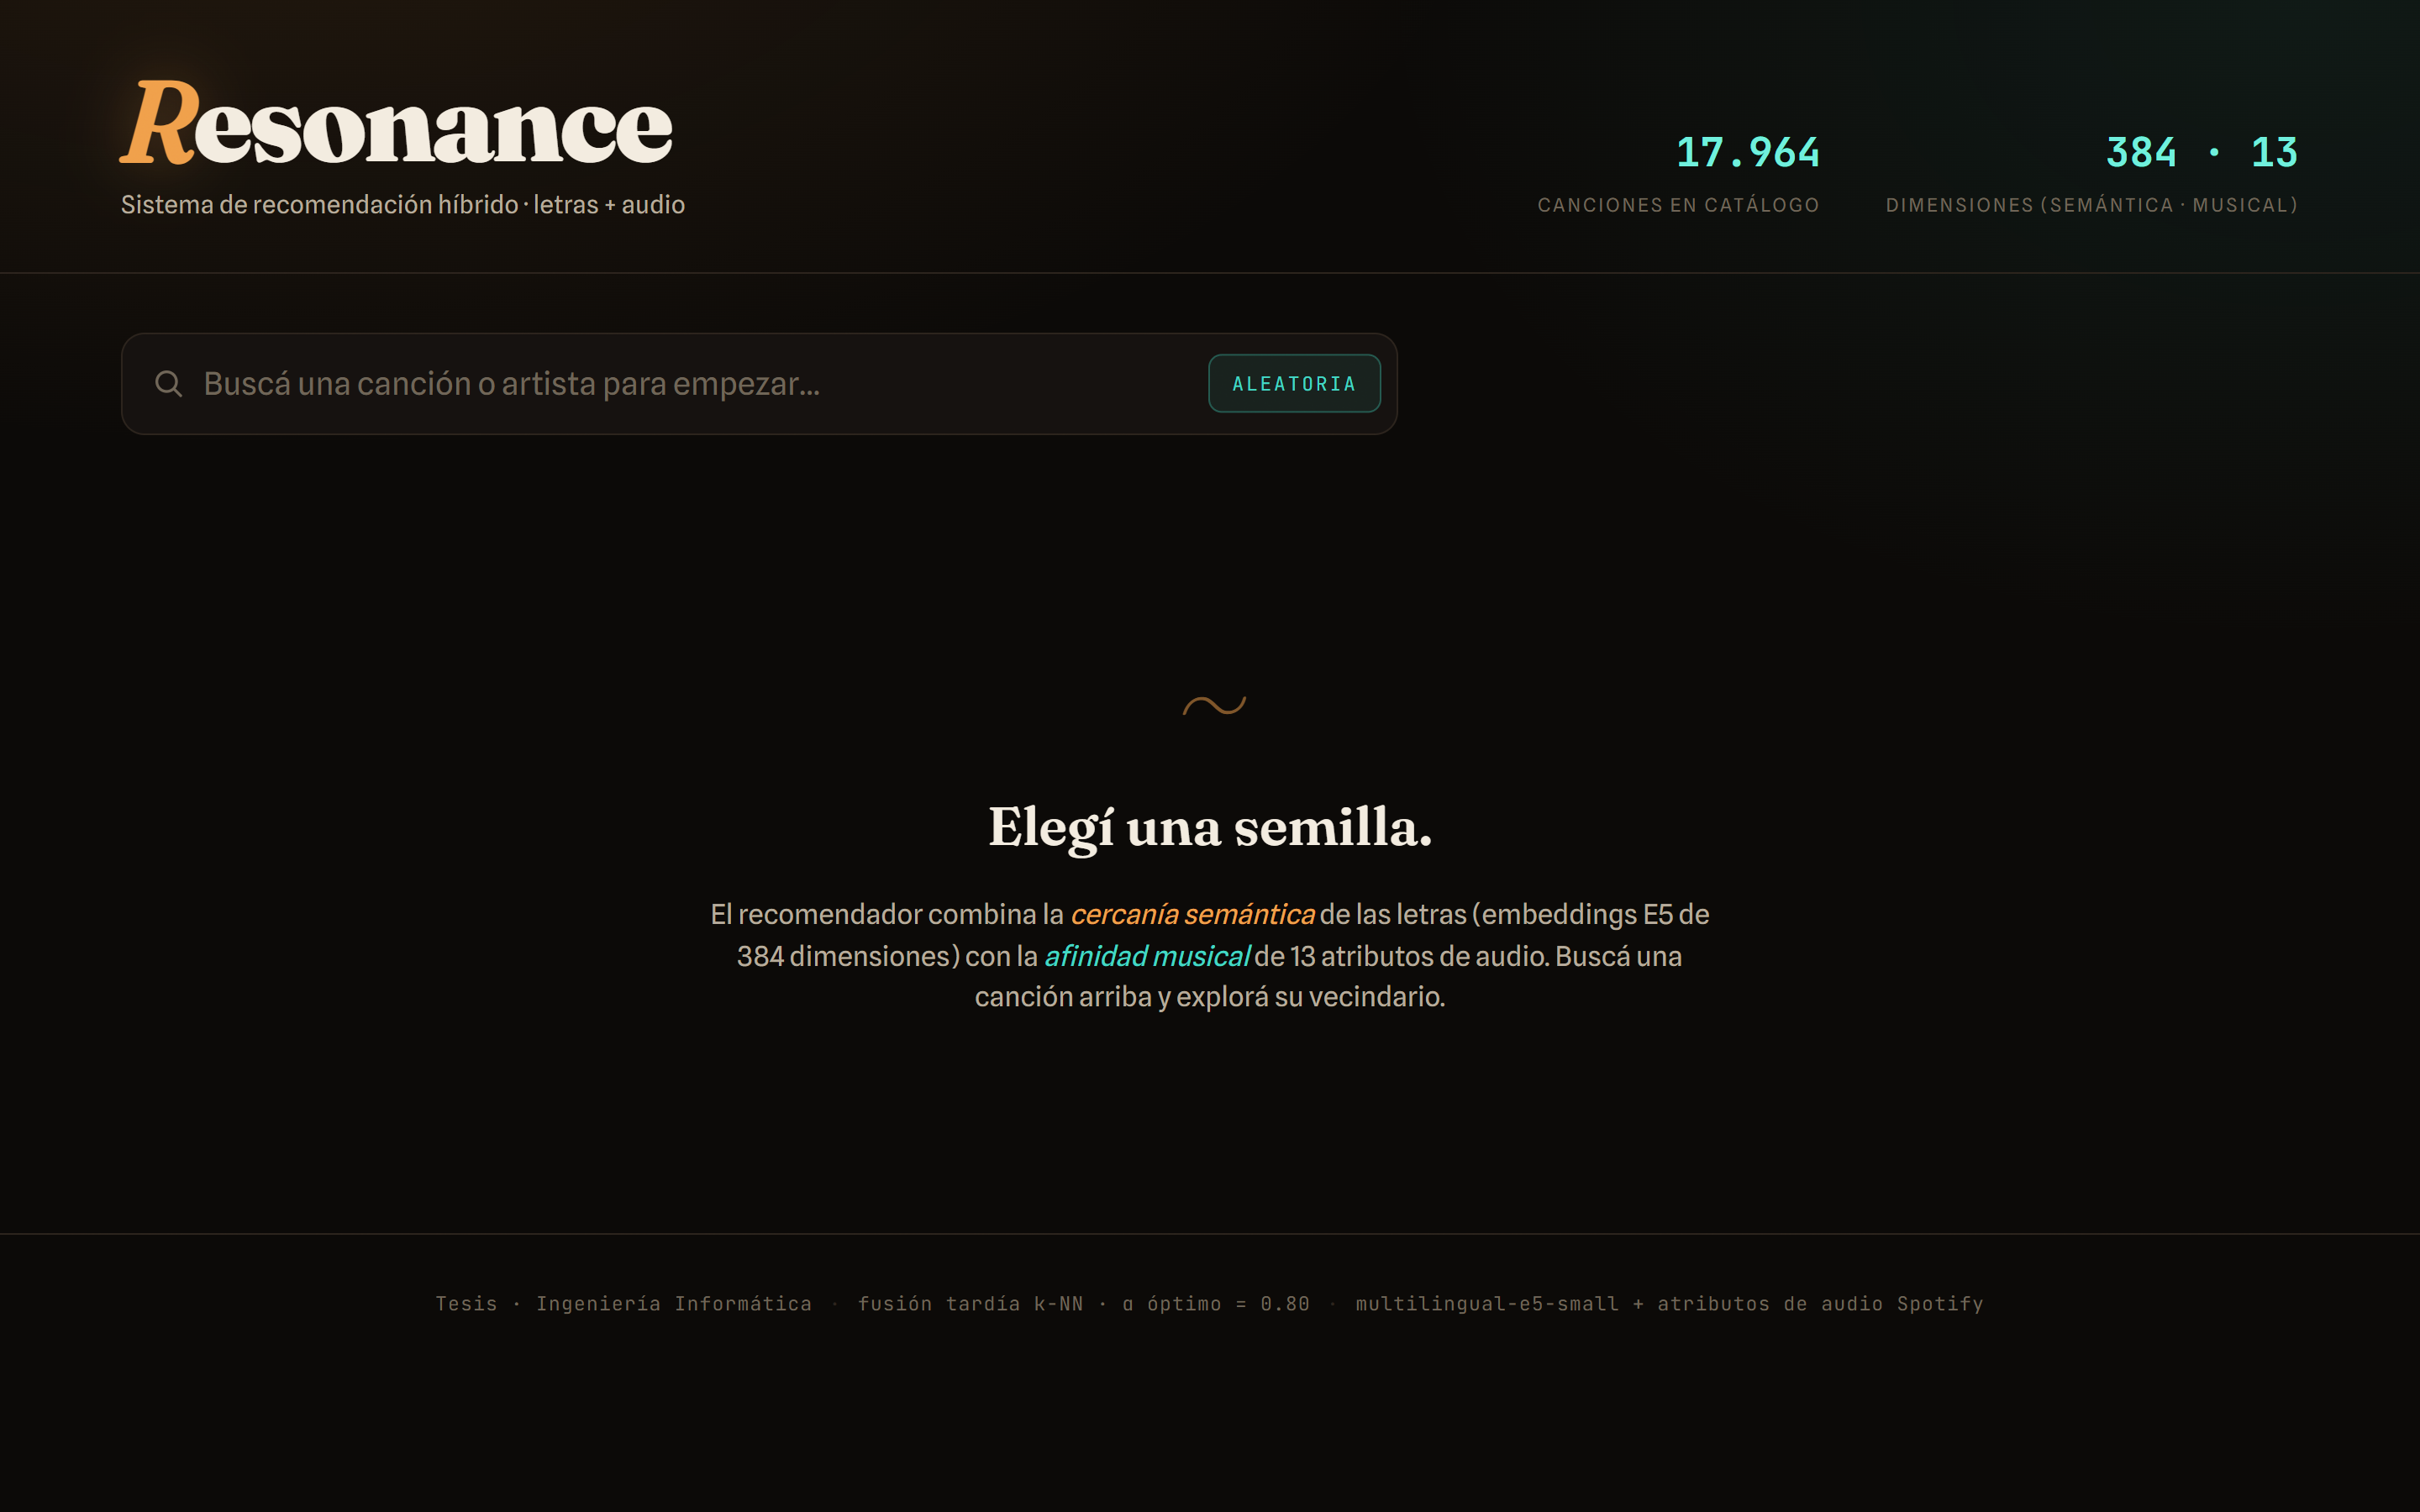
\includegraphics[width=0.95\textwidth]{figures/app/app_01_estado_inicial.png}
    \caption[Pantalla inicial de la aplicación web.]{Pantalla inicial. La cabecera informa el tamaño del catálogo y la dimensionalidad de ambas representaciones. Toda recomendación parte de una canción inicial que el usuario elige.}
    \label{fig:app_estado_inicial}
\end{figure}

\begin{figure}[htbp]
    \centering
    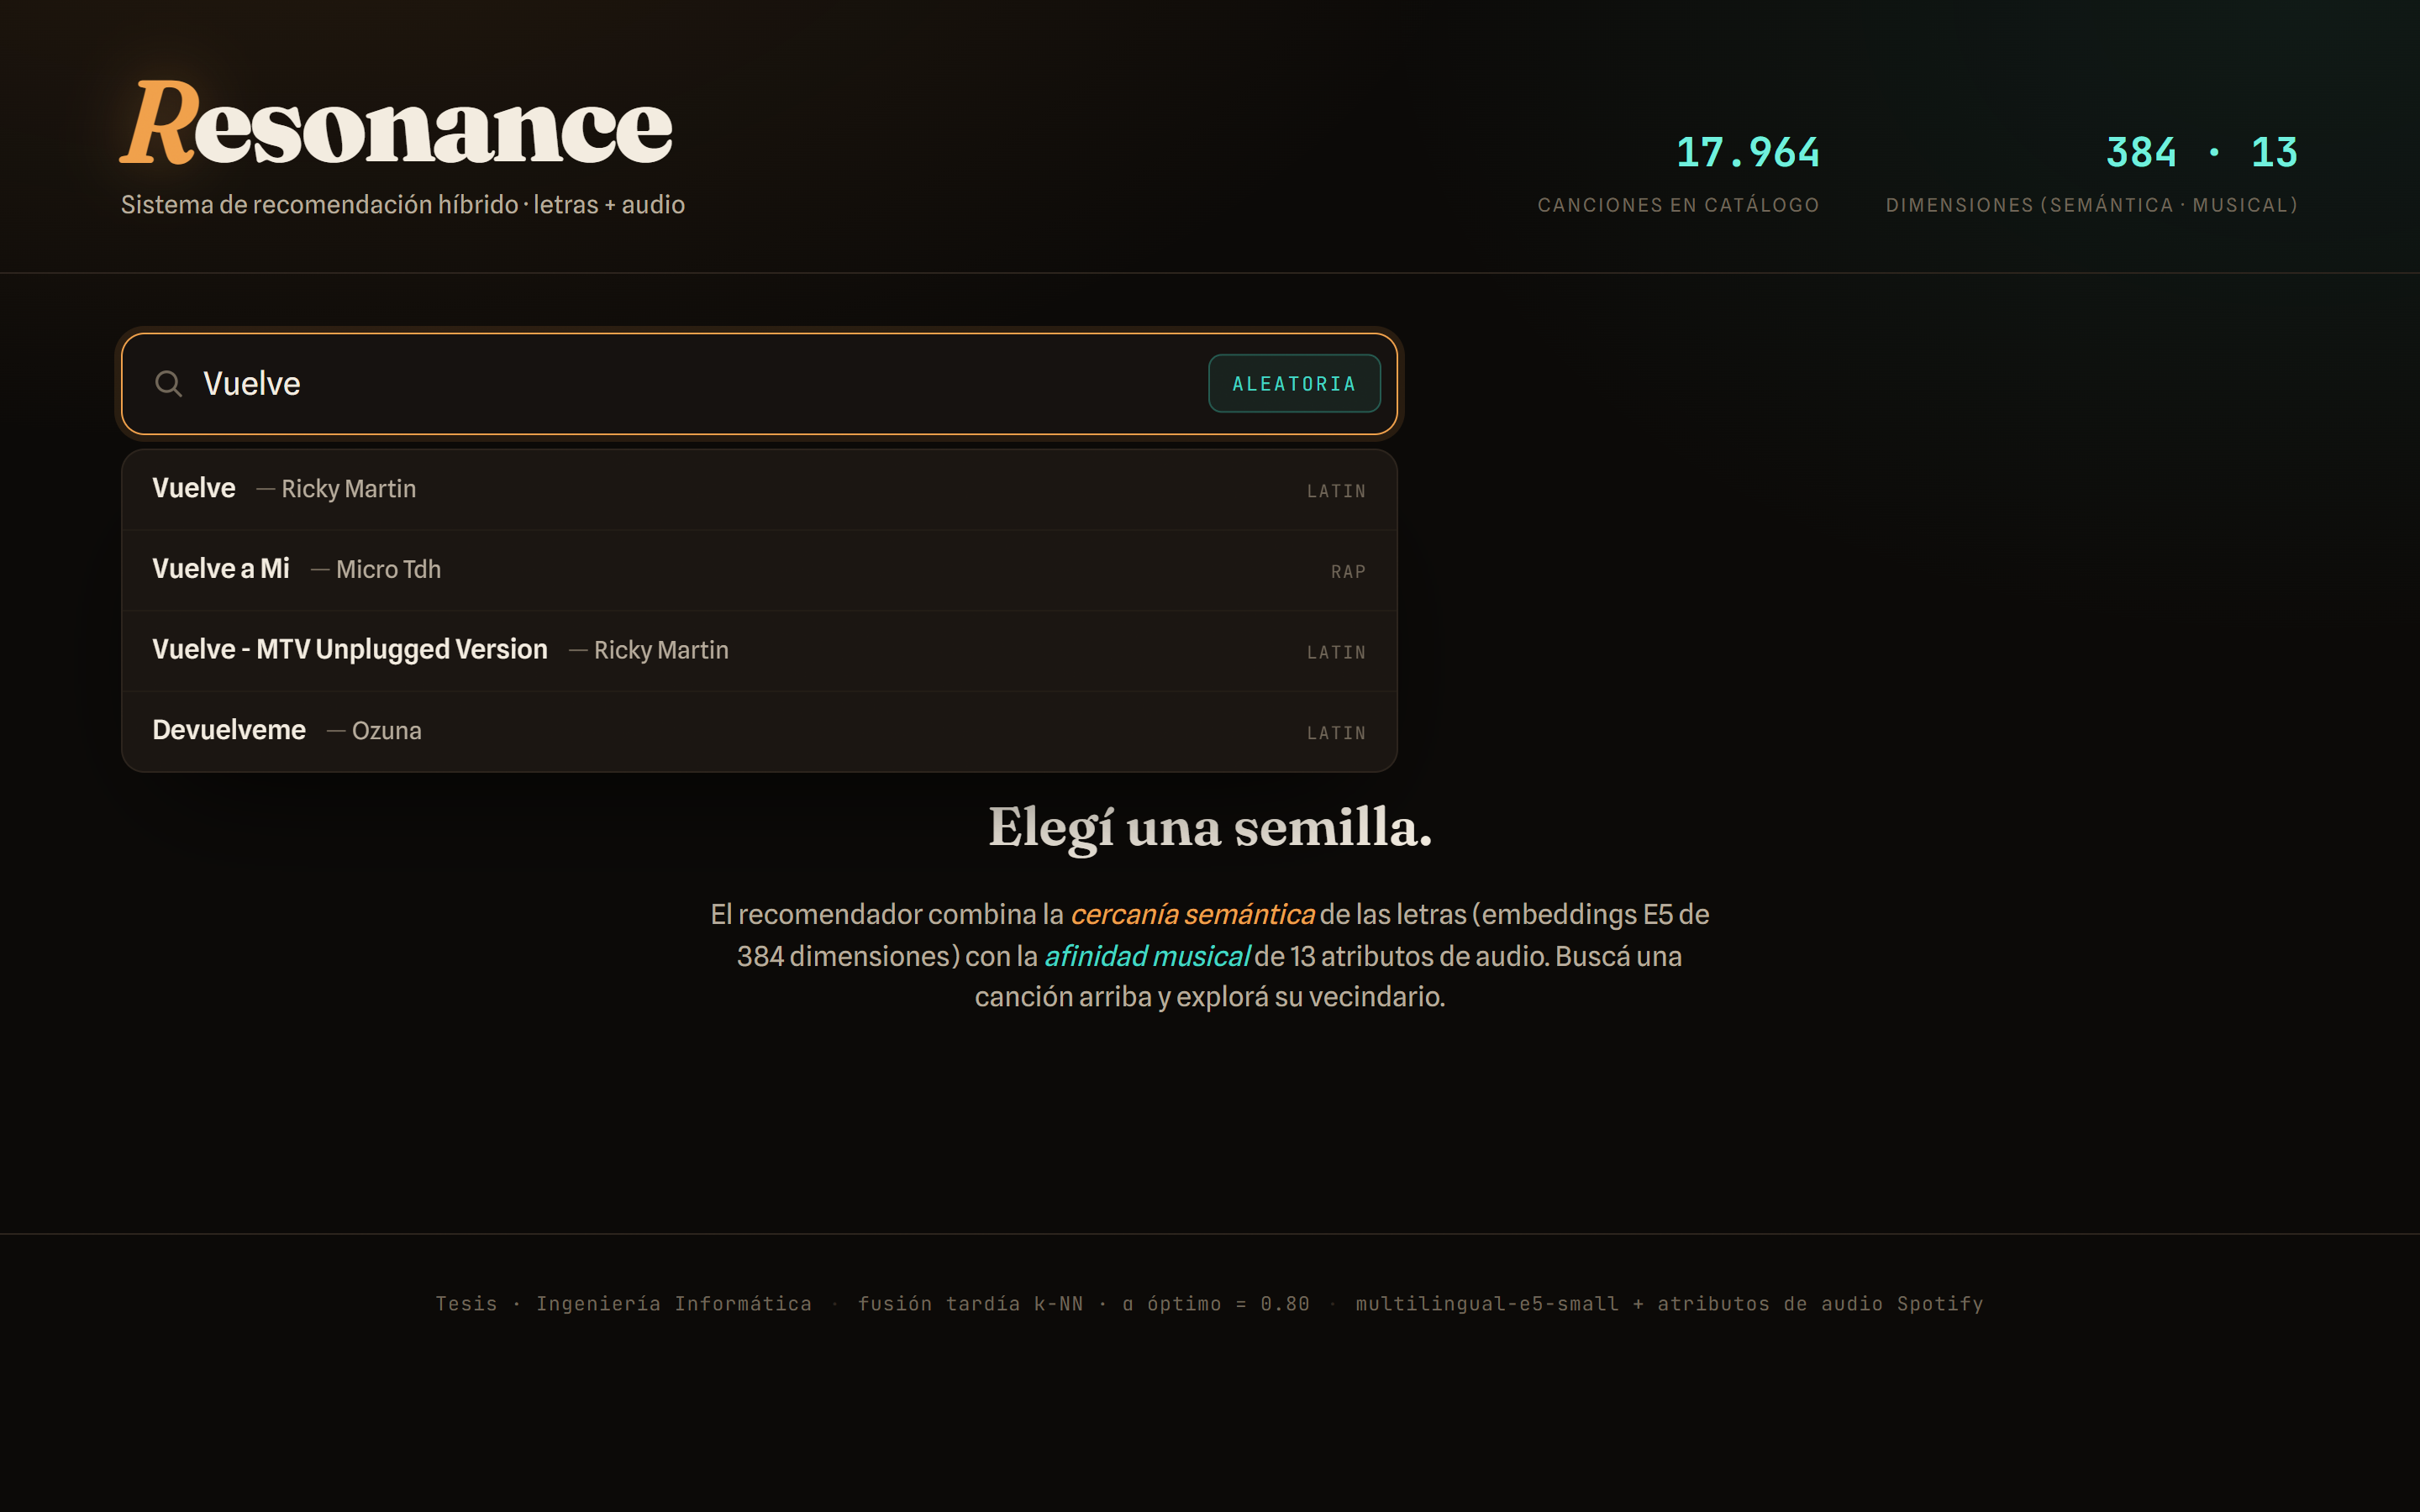
\includegraphics[width=0.95\textwidth]{figures/app/app_02_busqueda.png}
    \caption[Búsqueda incremental sobre el catálogo.]{Búsqueda por título o artista para la consulta \emph{Vuelve}. Las coincidencias por prefijo preceden a las internas, como \emph{Devuelveme}, y cada resultado se acompaña de su intérprete y su etiqueta de género.}
    \label{fig:app_busqueda}
\end{figure}

\FloatBarrier

Elegida la canción, el panel izquierdo presenta la canción consultada y los controles de la fusión, y el derecho su vecindario. La barra de cada recomendación descompone el puntaje.

\begin{figure}[htbp]
    \centering
    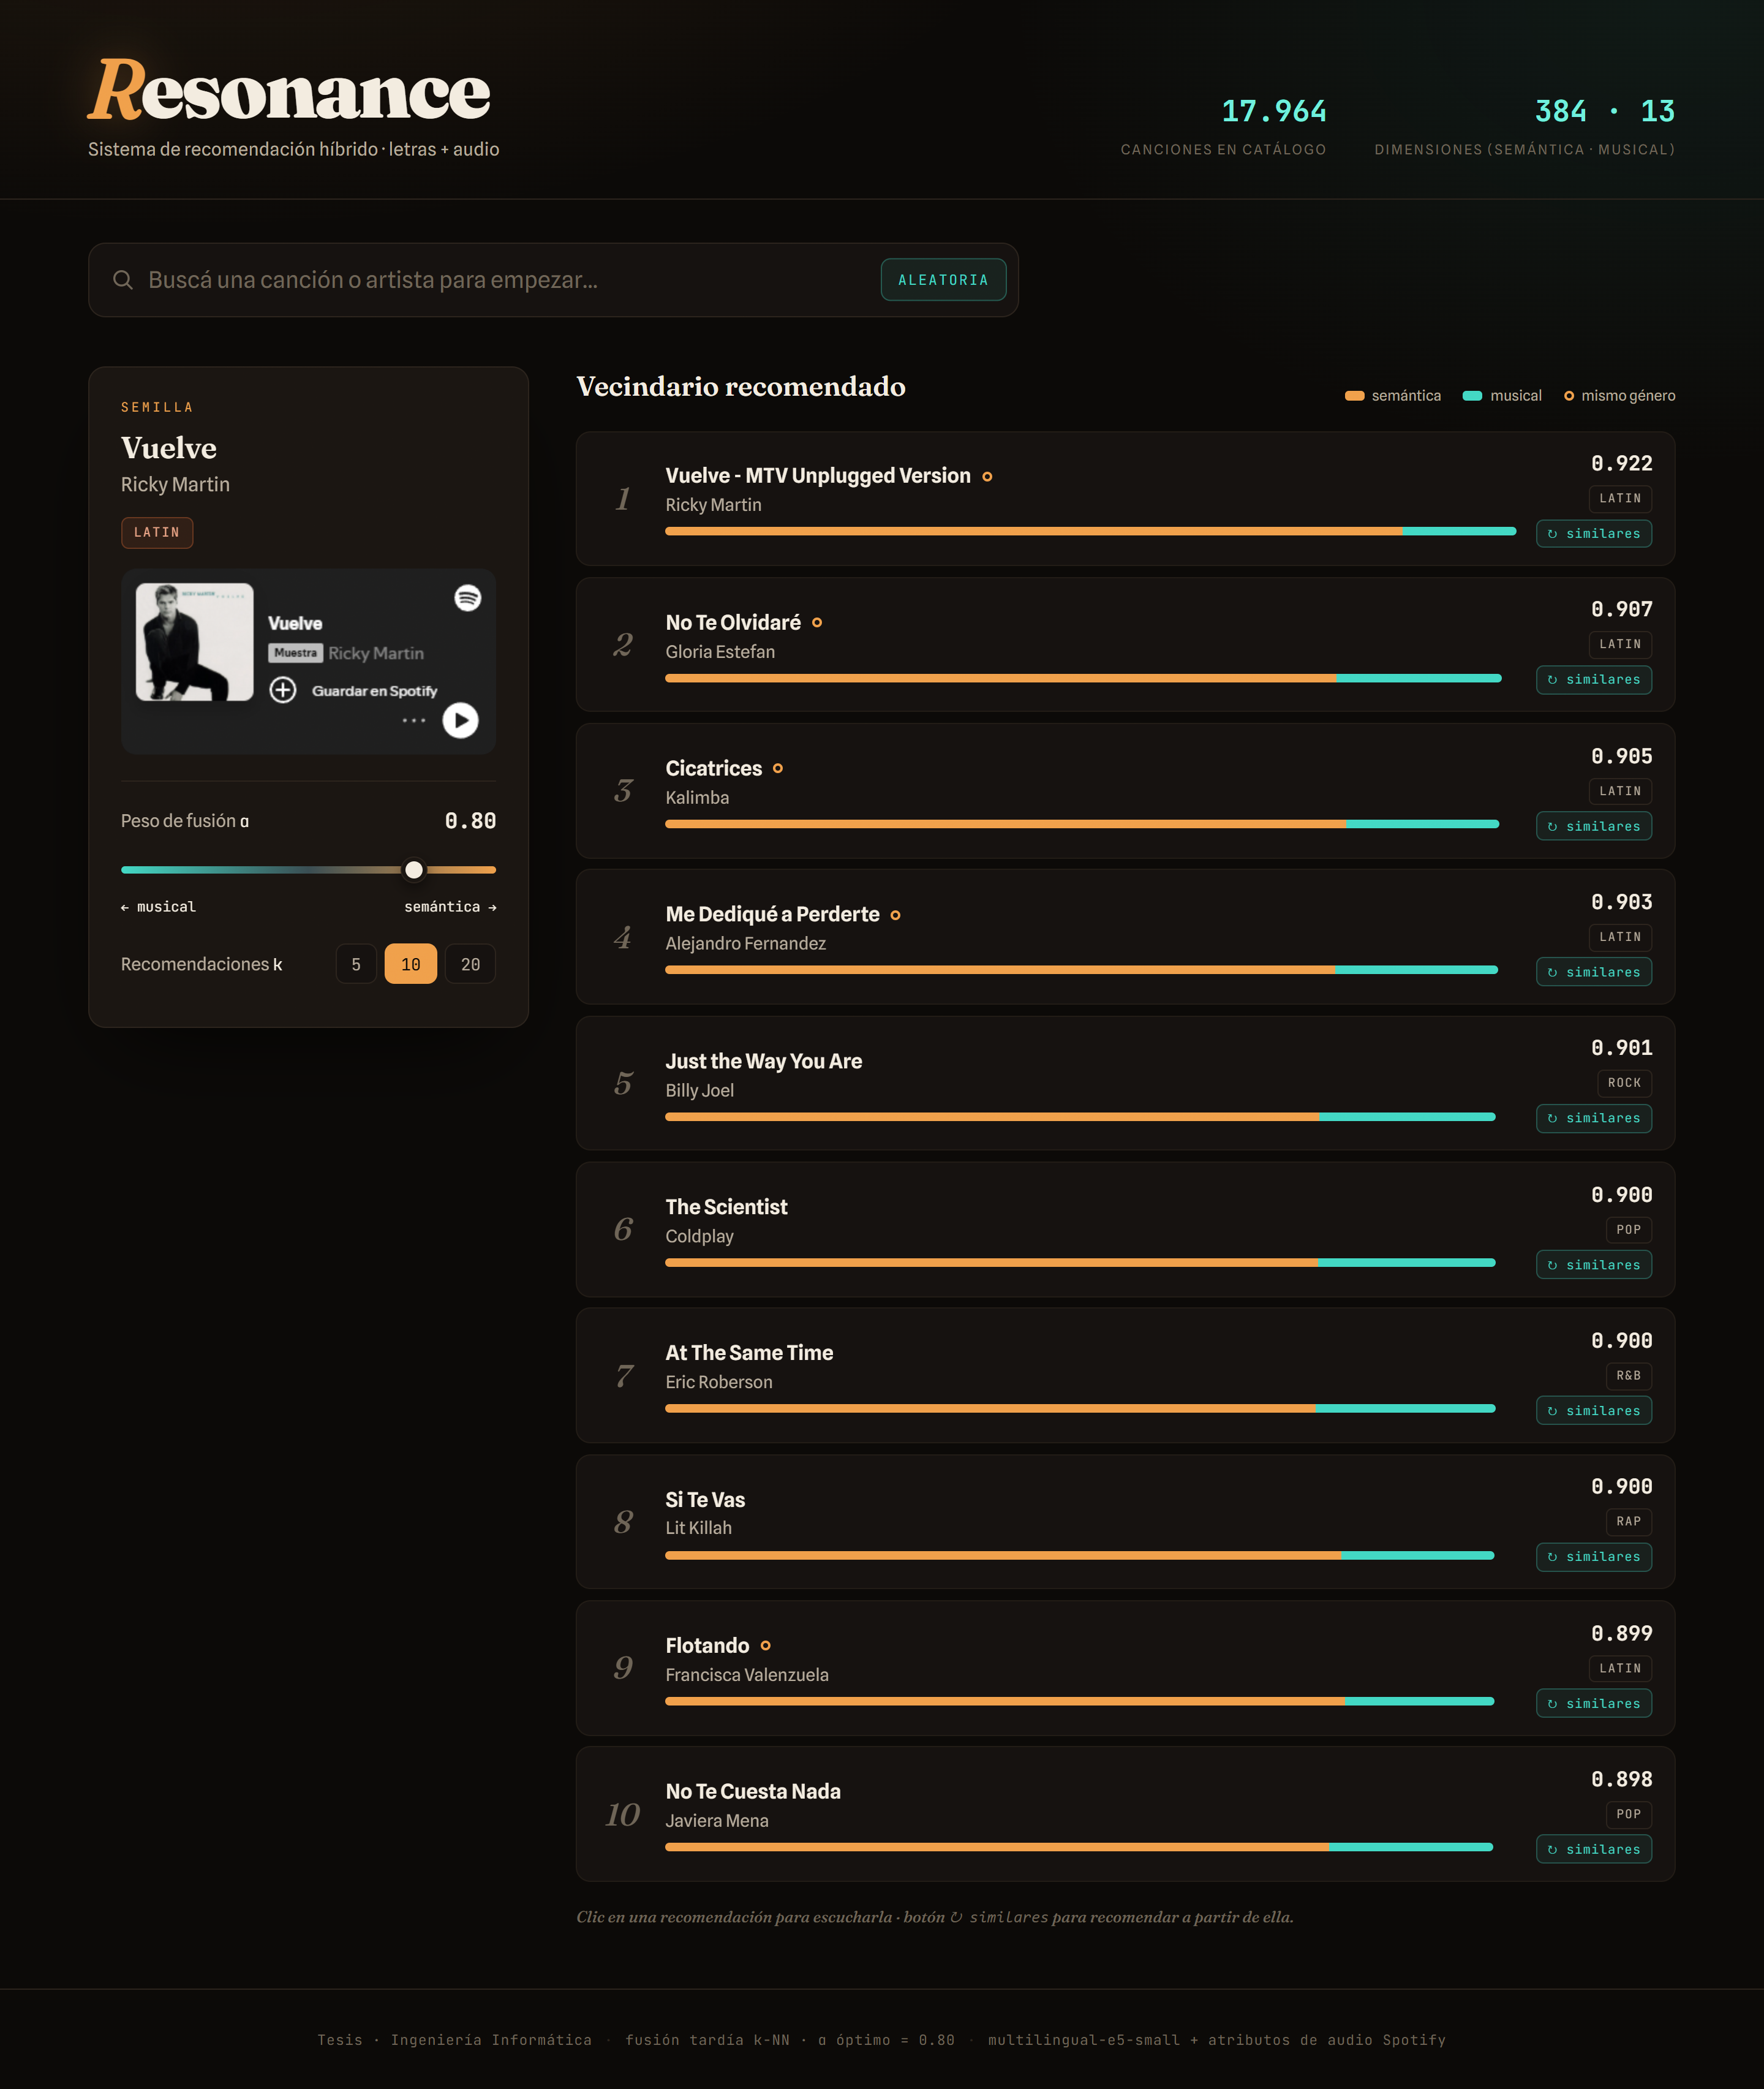
\includegraphics[width=0.80\textwidth]{figures/app/app_03_tablero_alpha080.png}
    \caption[Tablero de recomendación en la configuración de operación.]{Tablero para \emph{Vuelve} de Ricky Martin con $\alpha = 0{,}80$ y $k = 10$. Las cuatro primeras posiciones son canciones en español; la quinta y la sexta, baladas en inglés recuperadas por proximidad acústica.}
    \label{fig:app_tablero}
\end{figure}

\FloatBarrier

Las dos figuras siguientes recorren los extremos del control deslizante sobre la misma canción.

\begin{figure}[htbp]
    \centering
    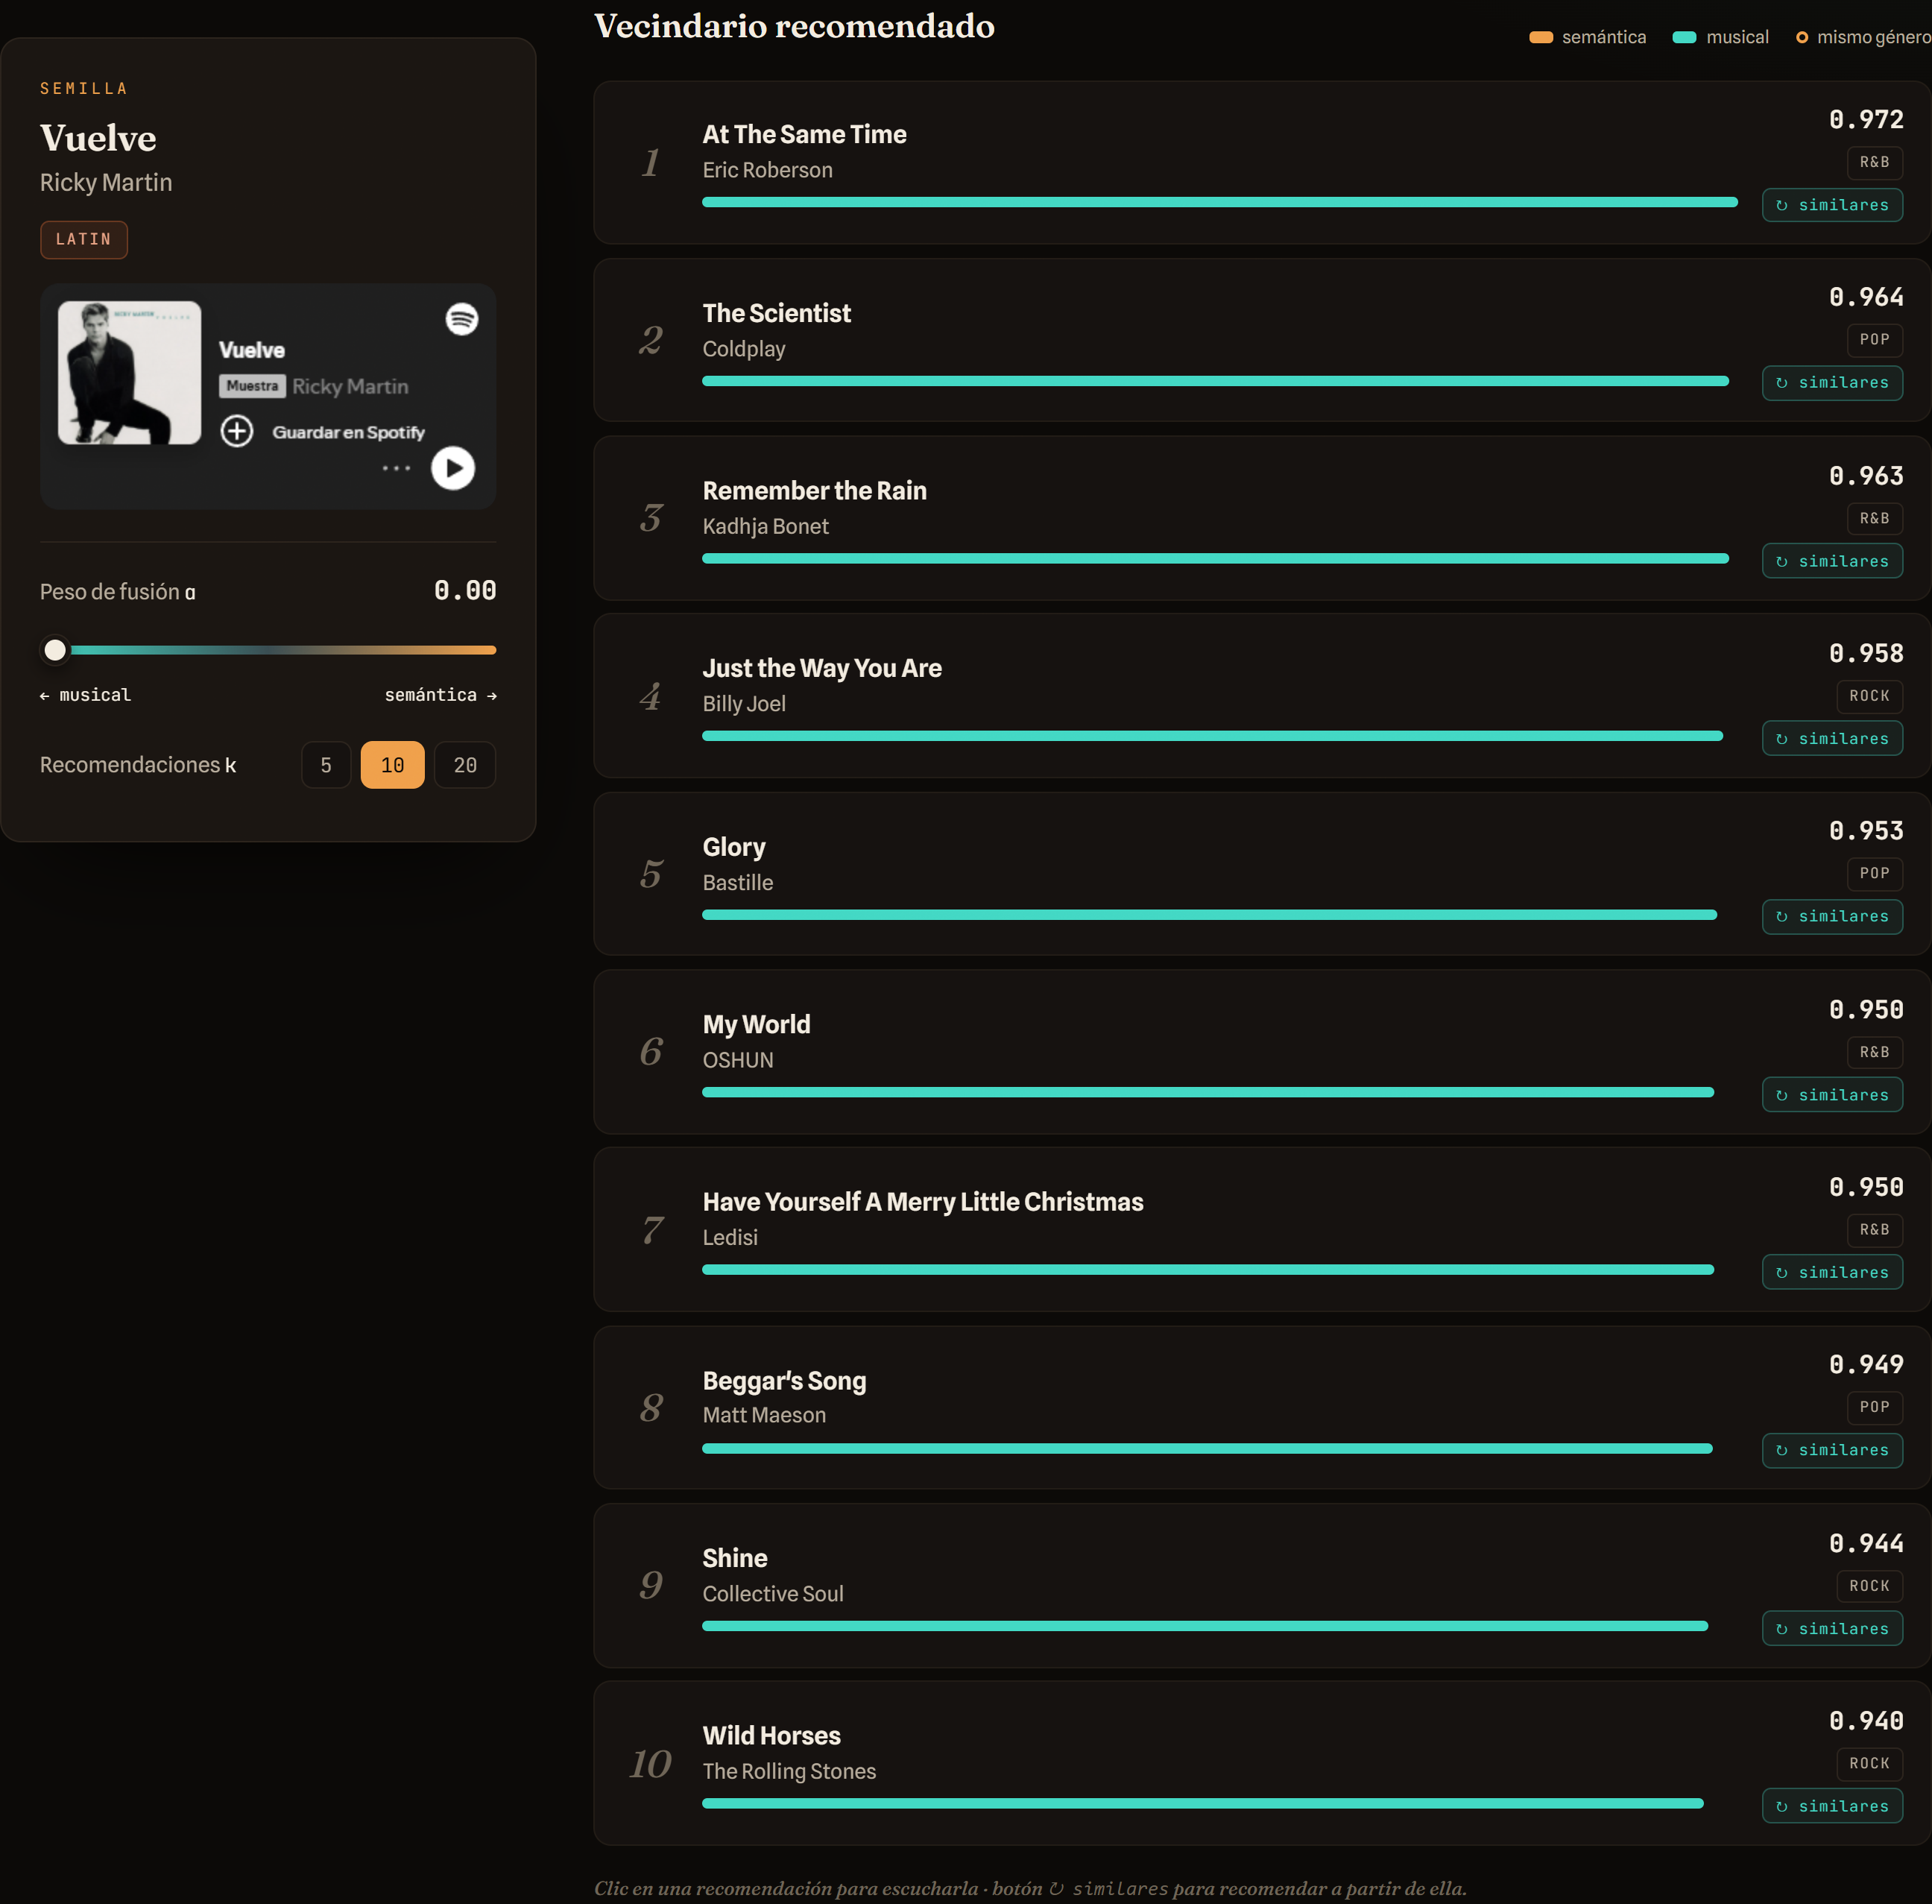
\includegraphics[width=0.85\textwidth]{figures/app/app_04_ablacion_alpha000.png}
    \caption[Recomendación puramente musical.]{Misma canción con $\alpha = 0{,}00$. Sin aporte semántico las barras carecen de segmento anaranjado y la lista, compuesta por afinidad acústica, pasa a ser enteramente anglófona.}
    \label{fig:app_ablacion_musical}
\end{figure}

\begin{figure}[htbp]
    \centering
    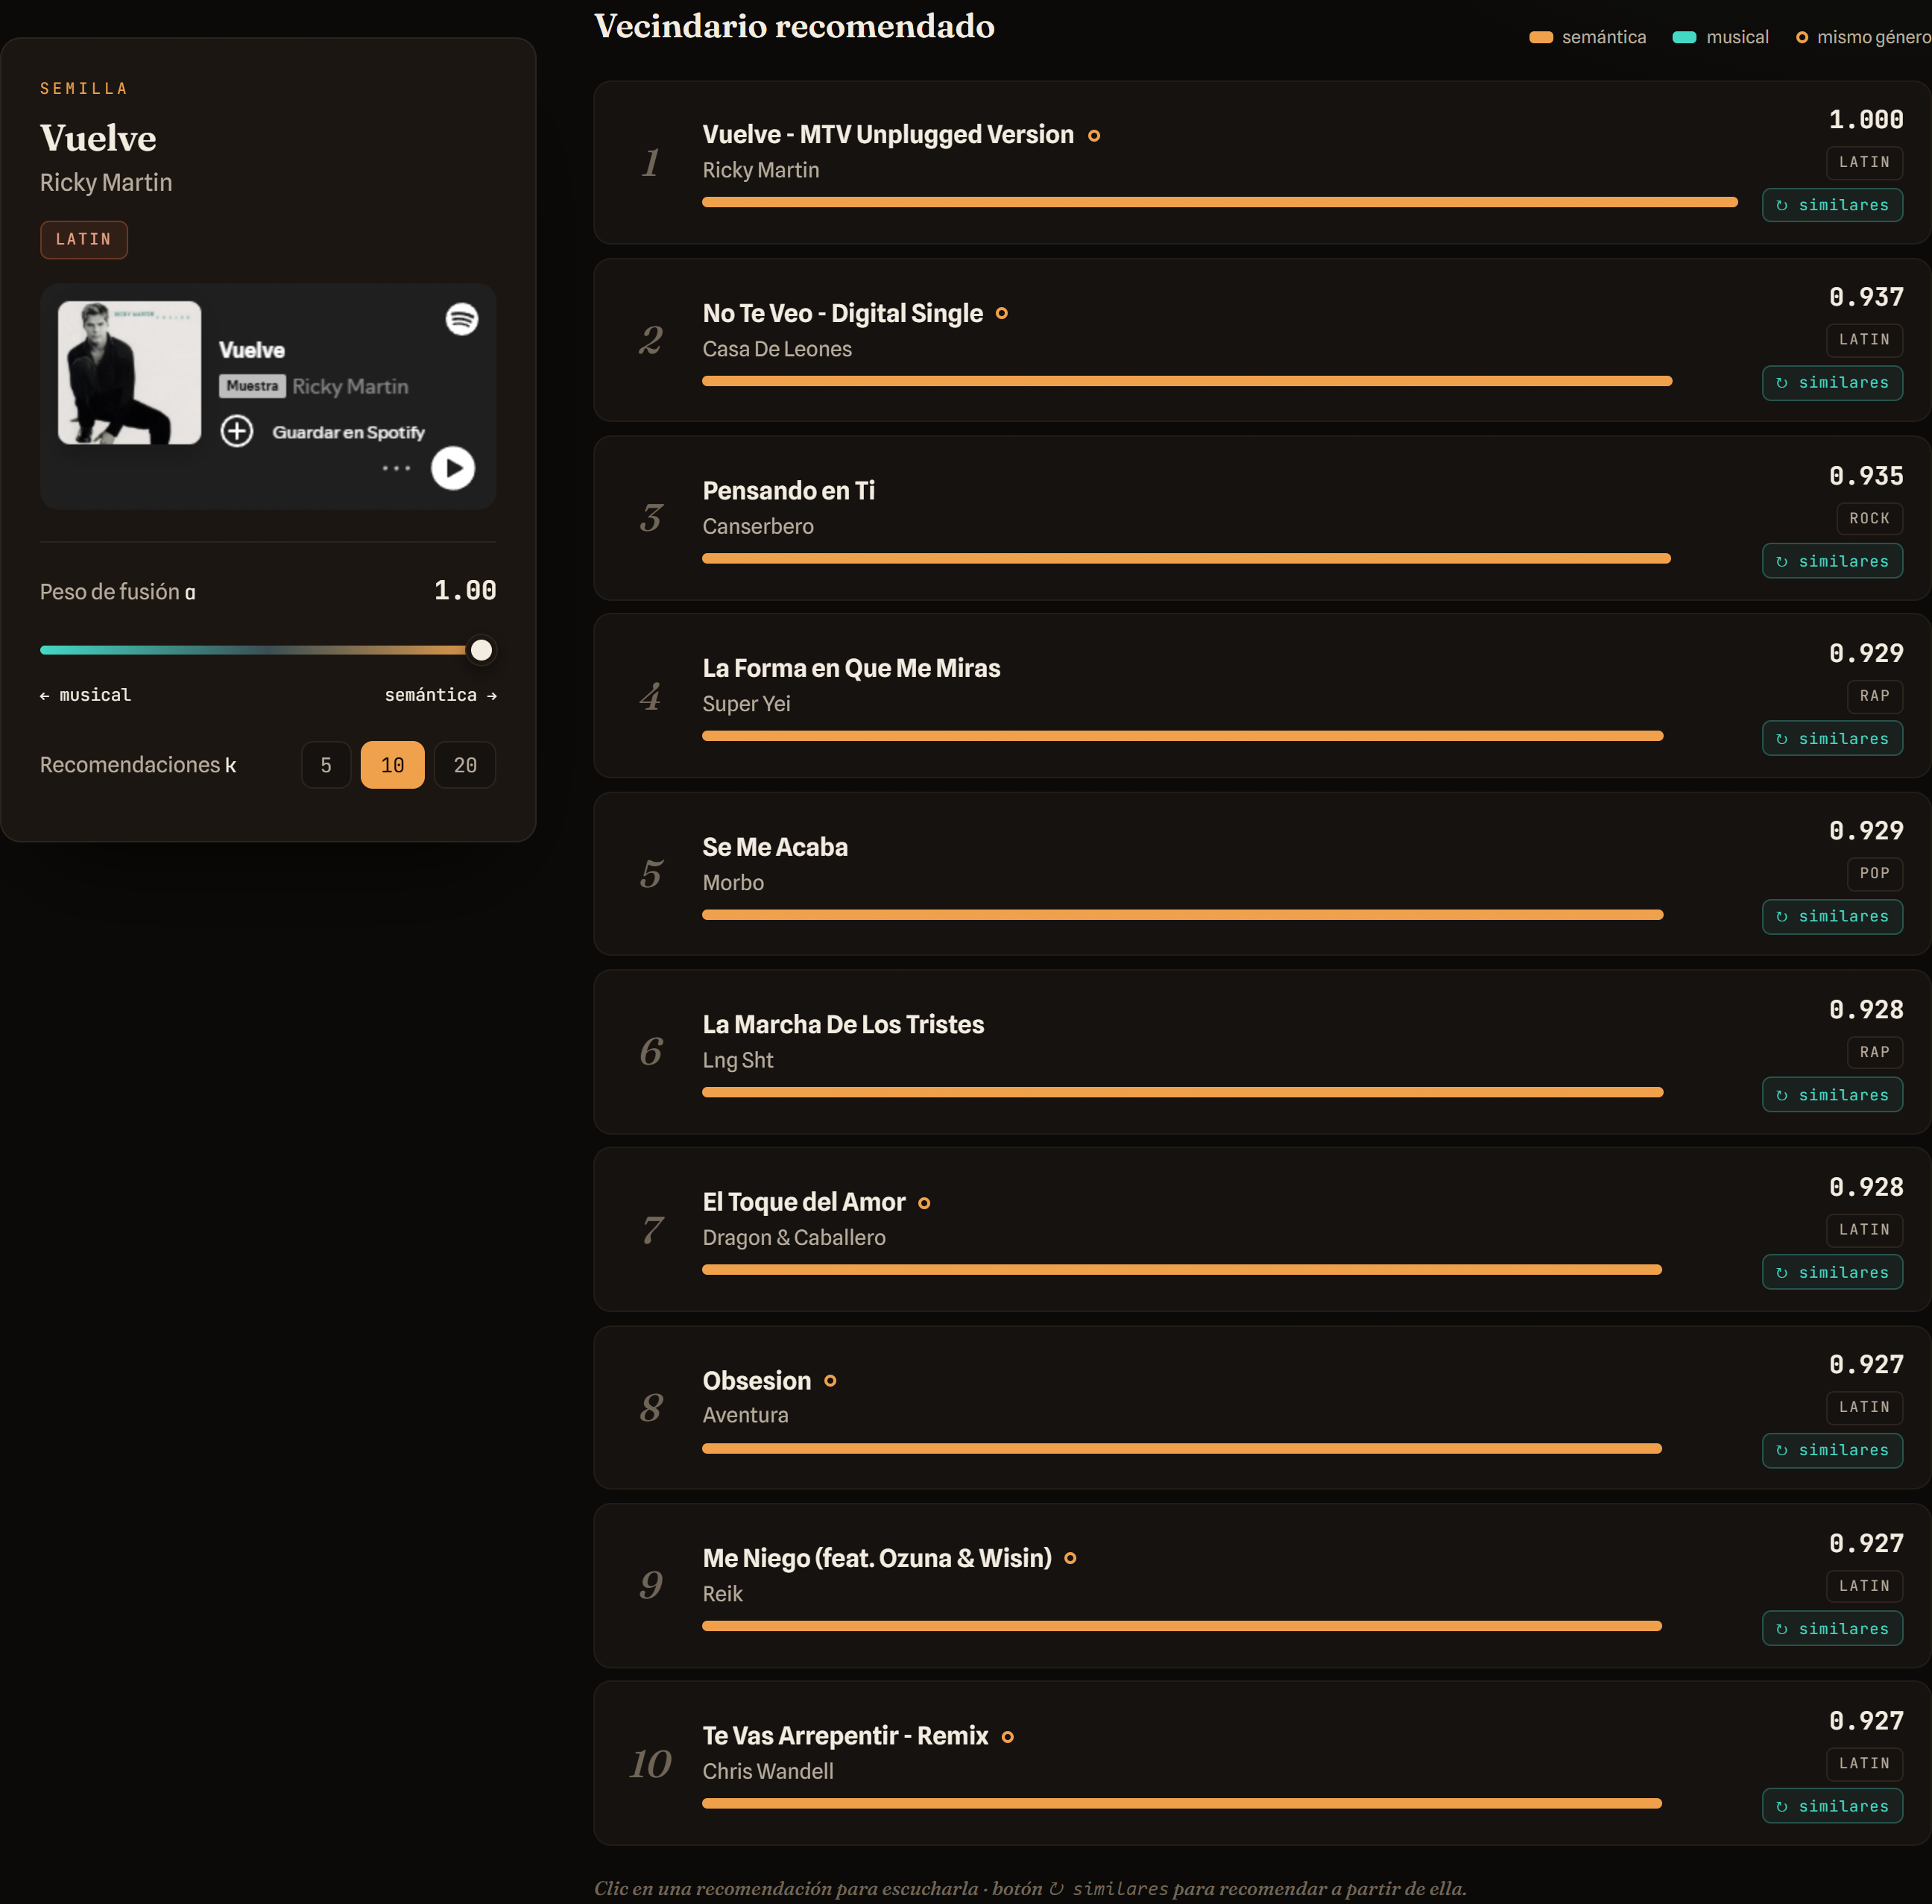
\includegraphics[width=0.85\textwidth]{figures/app/app_05_ablacion_alpha100.png}
    \caption[Recomendación puramente semántica.]{Misma canción con $\alpha = 1{,}00$. La lista resulta enteramente en español pero de géneros dispares, lo que evidencia que el espacio semántico segmenta por idioma. La versión acústica encabeza con puntaje $1{,}000$ por compartir la letra.}
    \label{fig:app_ablacion_semantica}
\end{figure}

\FloatBarrier

La longitud de la lista también es ajustable. Las dos figuras siguientes usan como canción inicial \emph{Lose Yourself} de Eminem.

\begin{figure}[htbp]
    \centering
    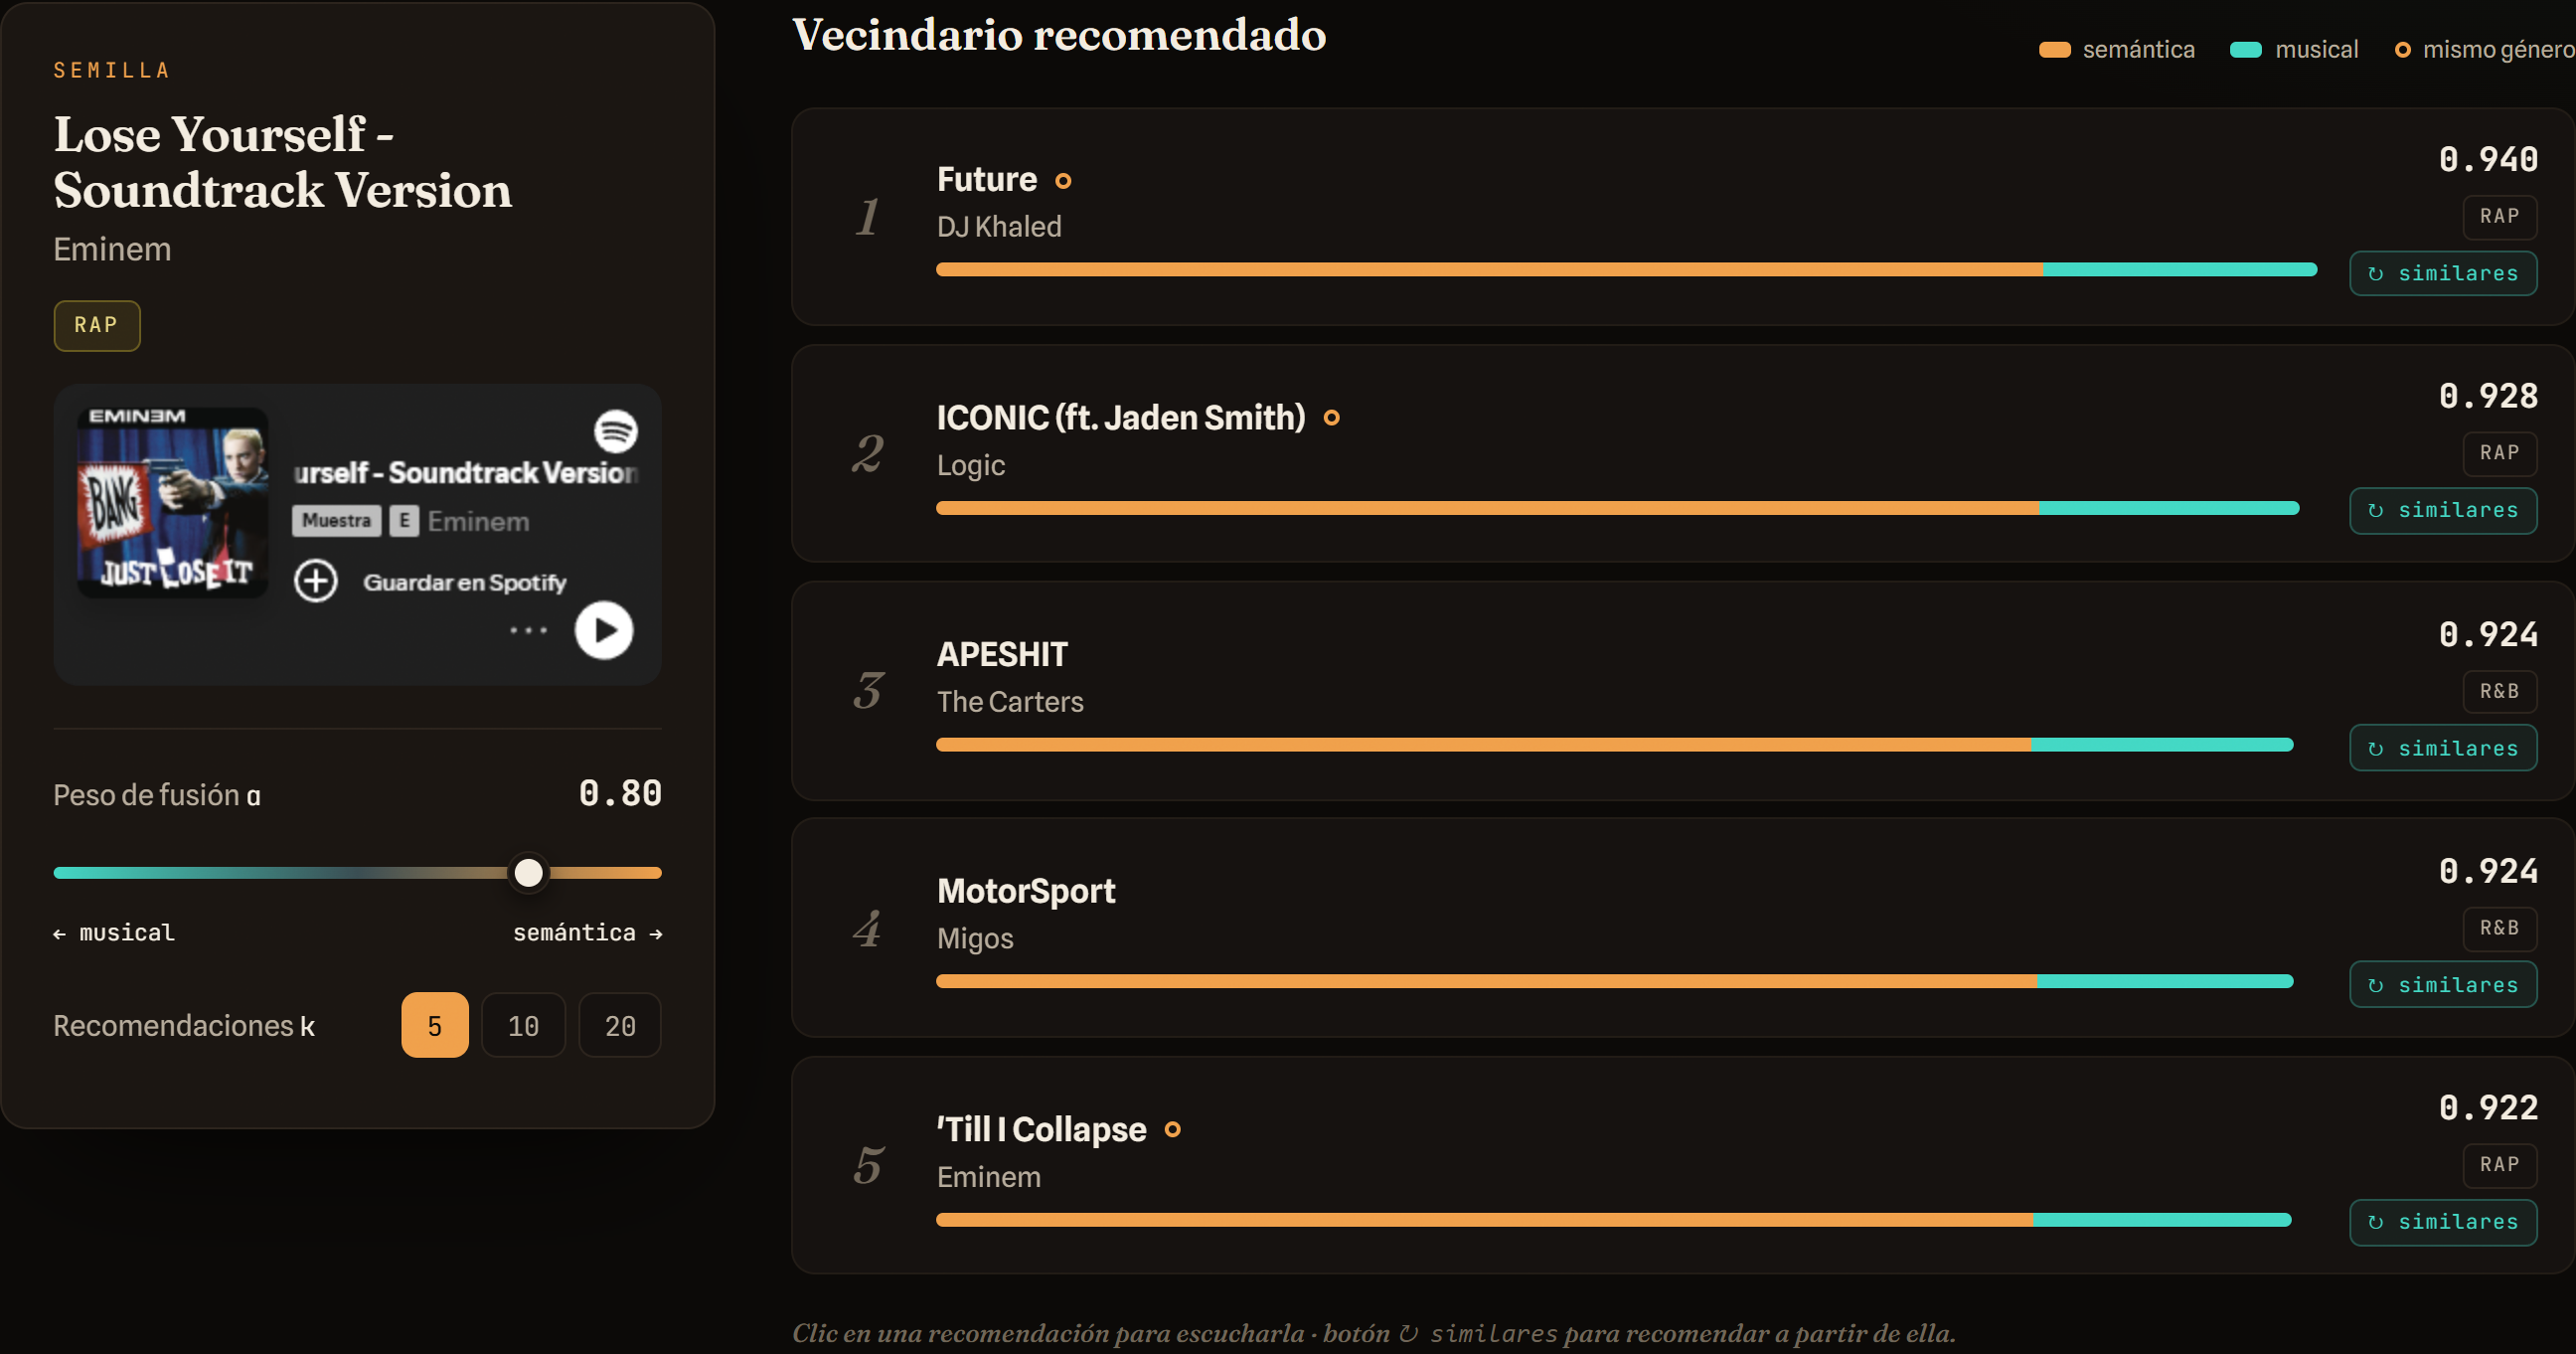
\includegraphics[width=0.95\textwidth]{figures/app/app_06_k5.png}
    \caption[Lista corta con depuración de duplicados.]{Vecindario con $k = 5$ y $\alpha = 0{,}80$. Las copias de la propia grabación presentes en el catálogo quedan excluidas de la lista mostrada.}
    \label{fig:app_k5}
\end{figure}

\begin{figure}[htbp]
    \centering
    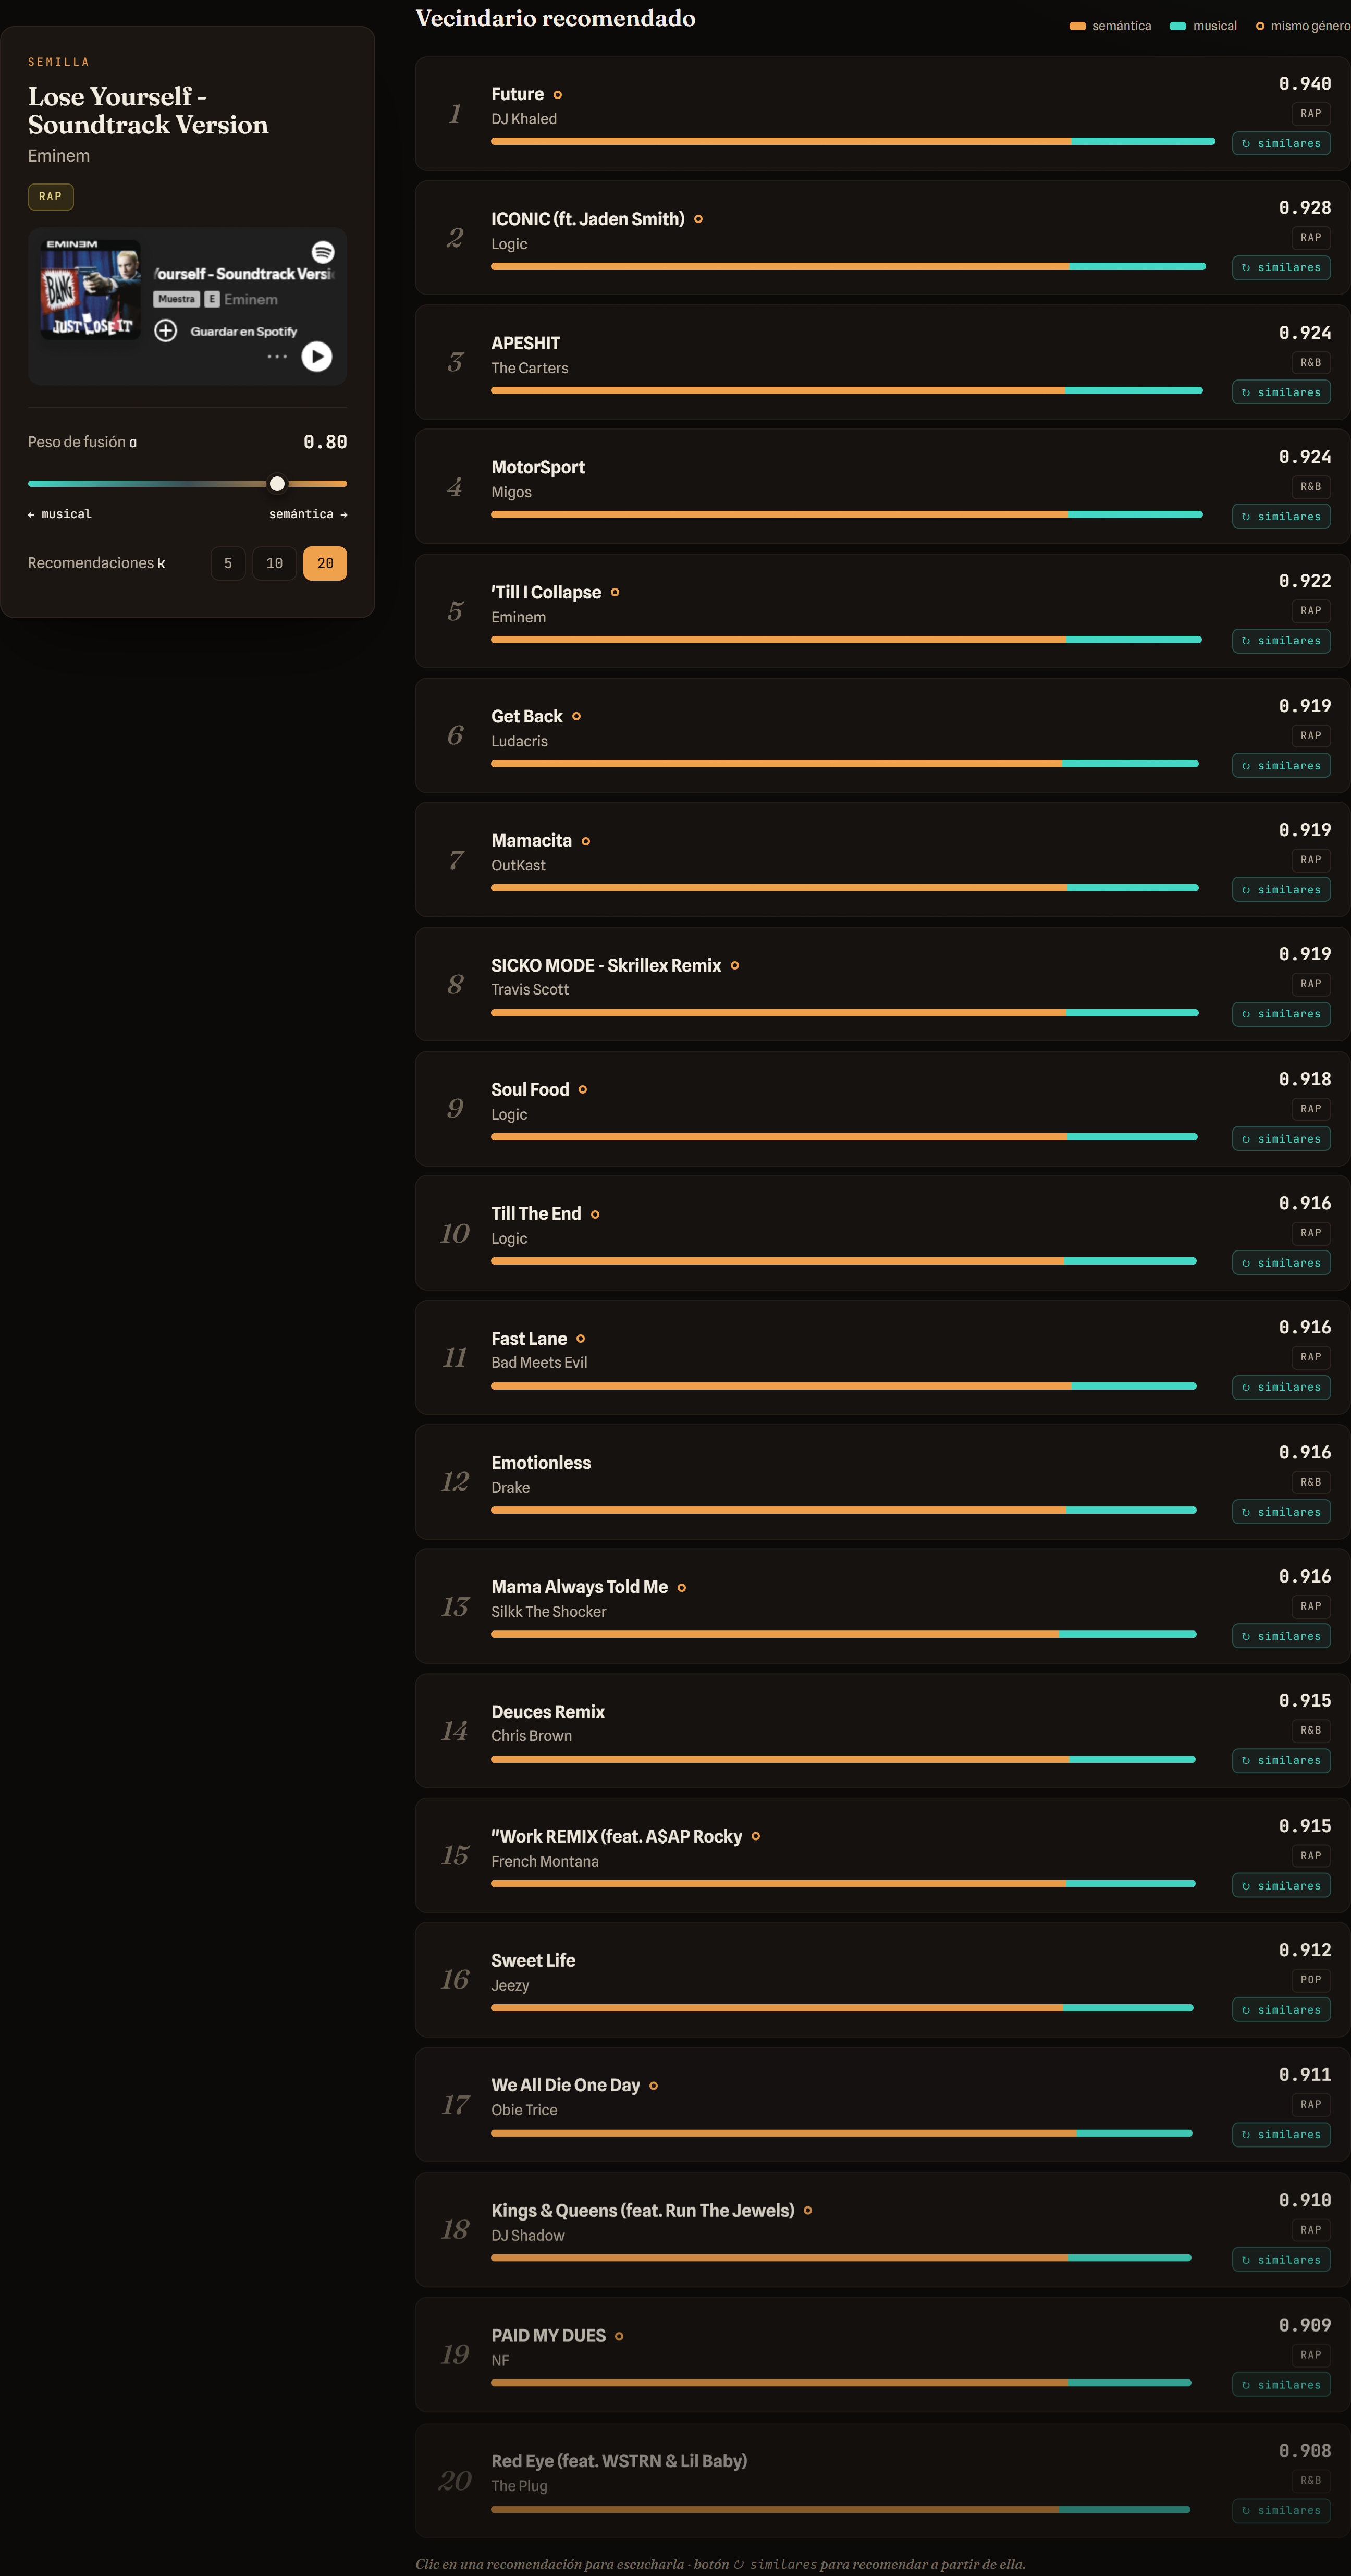
\includegraphics[height=0.82\textheight]{figures/app/app_07_k20.png}
    \caption[Lista extendida a veinte recomendaciones.]{Misma canción con $k = 20$. El puntaje desciende de forma continua a lo largo de la lista, de $0{,}940$ a $0{,}908$, sin un corte que delimite el vecindario.}
    \label{fig:app_k20}
\end{figure}

\FloatBarrier

Por último, la interfaz permite tomar una canción al azar, de modo que la demostración no dependa solamente de canciones elegidas.

\begin{figure}[htbp]
    \centering
    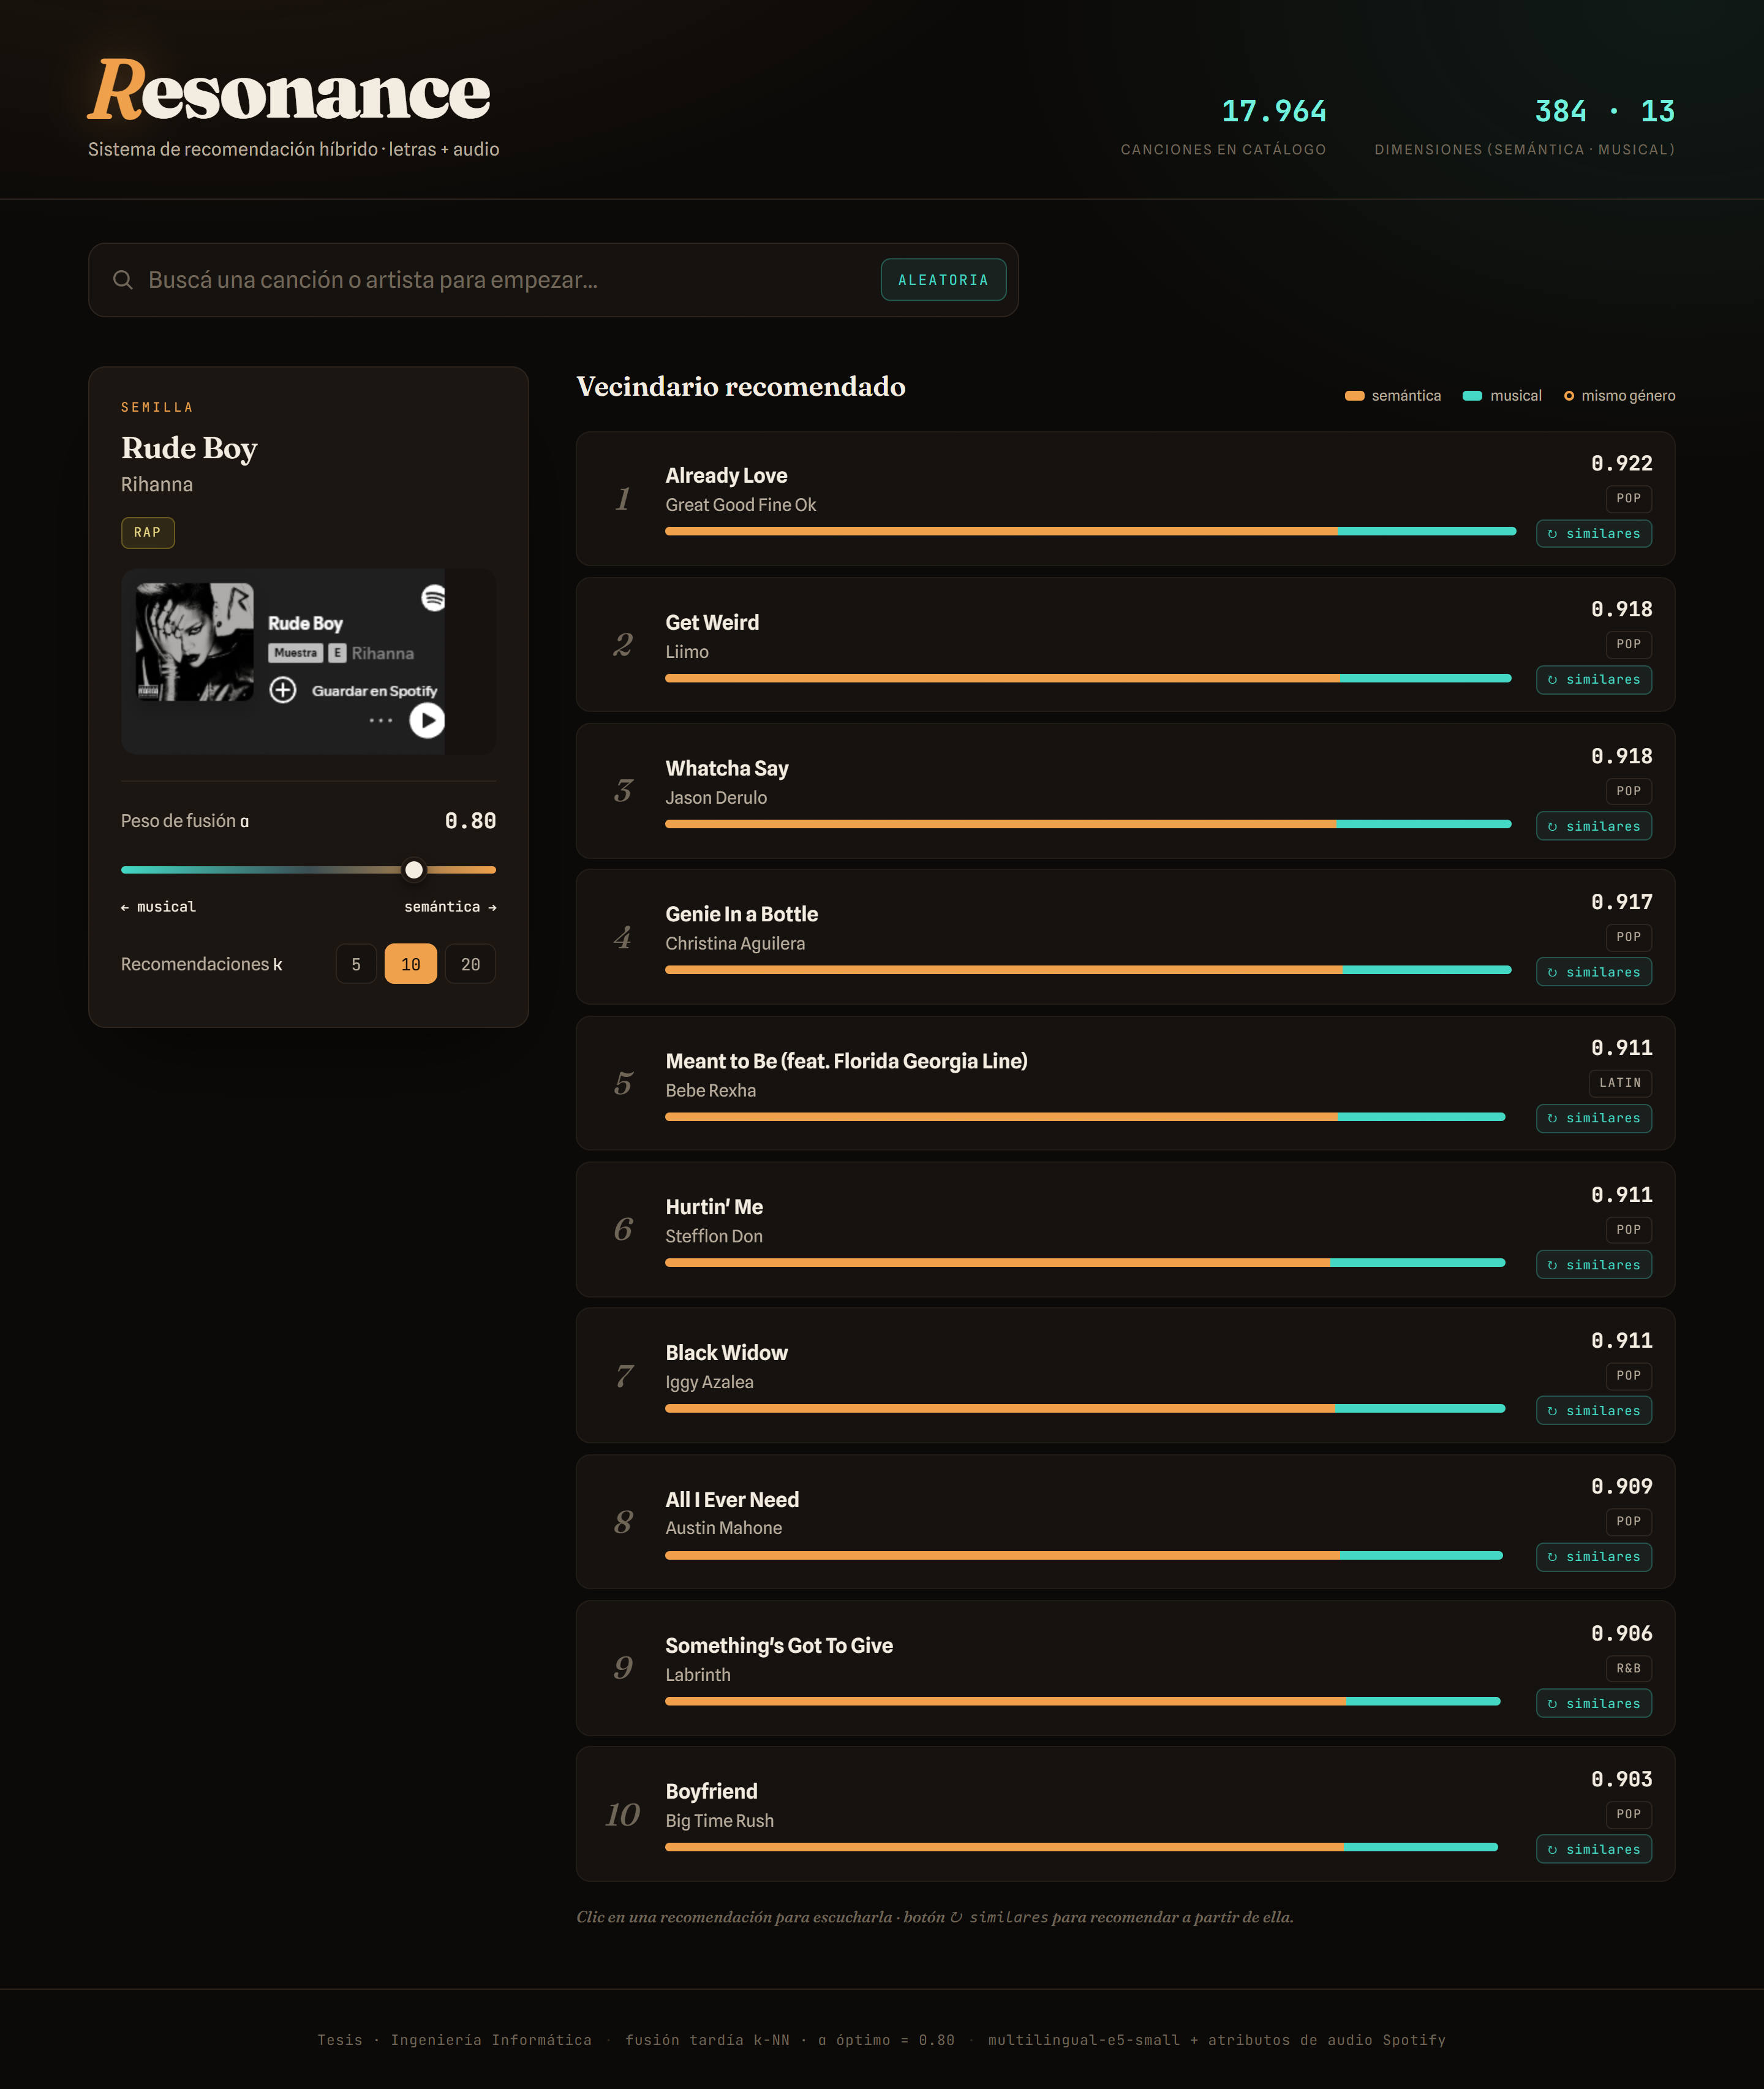
\includegraphics[width=0.80\textwidth]{figures/app/app_08_aleatoria.png}
    \caption[Recomendación a partir de una canción aleatoria.]{Vecindario de \emph{Rude Boy} de Rihanna, obtenida por selección aleatoria. Las recomendaciones son coherentes en estilo pese a que ninguna comparte la etiqueta de género de la canción, que el conjunto de datos registra como rap.}
    \label{fig:app_aleatoria}
\end{figure}
